\section{Algorithm Output and Testing}
% Writing code: Make it run. Make it correct. Make it fast.
My implementation of the linear-Gaussian binary latent feature model with the IBP prior generates the results in images and traceplots. The simulated dataset contains four latent features (see Figure~\ref{fig:images}), but my code reveals five latent features in Figure~\ref{fig:imageresults}, three of which are the linear combinations of two latent features. The traceplots in Figure~\ref{fig:plotresults} show my Gibbs sampler is converging: $K_+$ fluctuates between 5 and 8; the IBP parameter $\alpha$ is within (0.5,1.5); $\sigma_X$ converges to the true value 0.5; $\sigma_A$ oscillates around 0.4. A total of 1000 Gibbs sampling iterations were performed, but the values started to converge at the 100th iteration.\\

I also performed in-line code testing by various methods. In the IBP prior, the \texttt{assert} command is used to verify $\frac{m_k}{i}$ to be a probability, i.e. between 0 and 1 -- because the $i$th ($i > 2)$ customer takes dish $k$ with probability $\frac{m_k}{i}$ in the IBP algorithm. In many parts of my code, I used \texttt{np.dot} from \texttt{numpy} to do matrix multiplications even when the size of matrices is small, instead of multiplying each column/row one by one. In this way, the dimensions in matrix multiplications are assured to match each other.

\begin{figure}[!ht]
\centering
    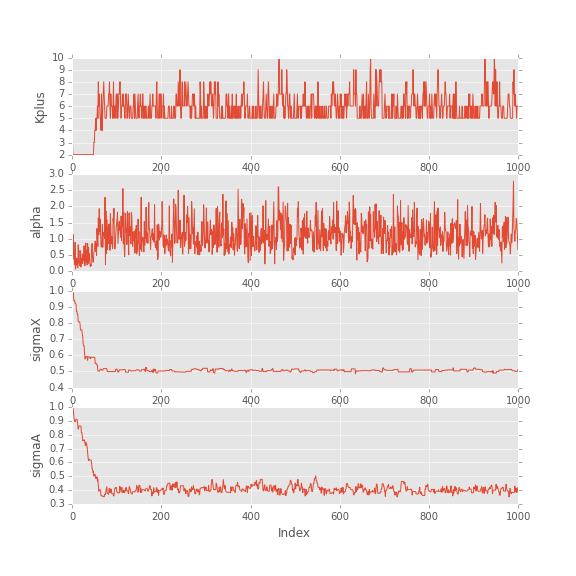
\includegraphics[width=0.65\linewidth]{IBP_plot_results.png}
    \vspace{-20pt}
    \caption{The traceplots for $K_+, \alpha, \sigma_X, \sigma_A$}
    \label{fig:plotresults}
\end{figure}

\begin{figure}[!ht]
\centering
    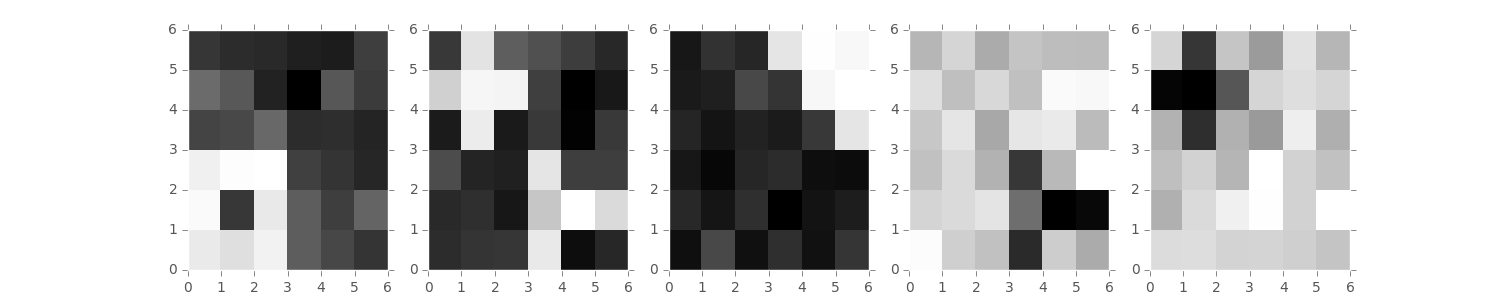
\includegraphics[width=\linewidth]{IBP_image_results.png}
    \caption{Simulated dataset: My results}
    \label{fig:imageresults}
\end{figure}